\section{方法：Civitas Economica 框架}
\label{sec:method}

Civitas Economica 在同一时钟下连接人与人的联系、人与群体的相互影响，以及群体与社会尺度的市场结果。图~\ref{fig:overview} 从可见观察出发，经估值与订单推进到结算，再将价格与持仓反馈至下一步。设主体总数为 $N$，主体索引为 $i,j\in\{1,\dots,N\}$，仿真步为 $t\in\{1,\dots,T\}$。截断算子为 $\clip(x,l,u)=\max(l,\min(u,x))$，标准 Logistic 函数为 $\sigma(x)=(1+e^{-x})^{-1}$。市场交易单一风险资产与无风险现金。每张订单均以可用现金或可卖持仓为上限，市场禁止无抵押借贷和裸卖空。

\begin{figure*}[t]
  \centering
  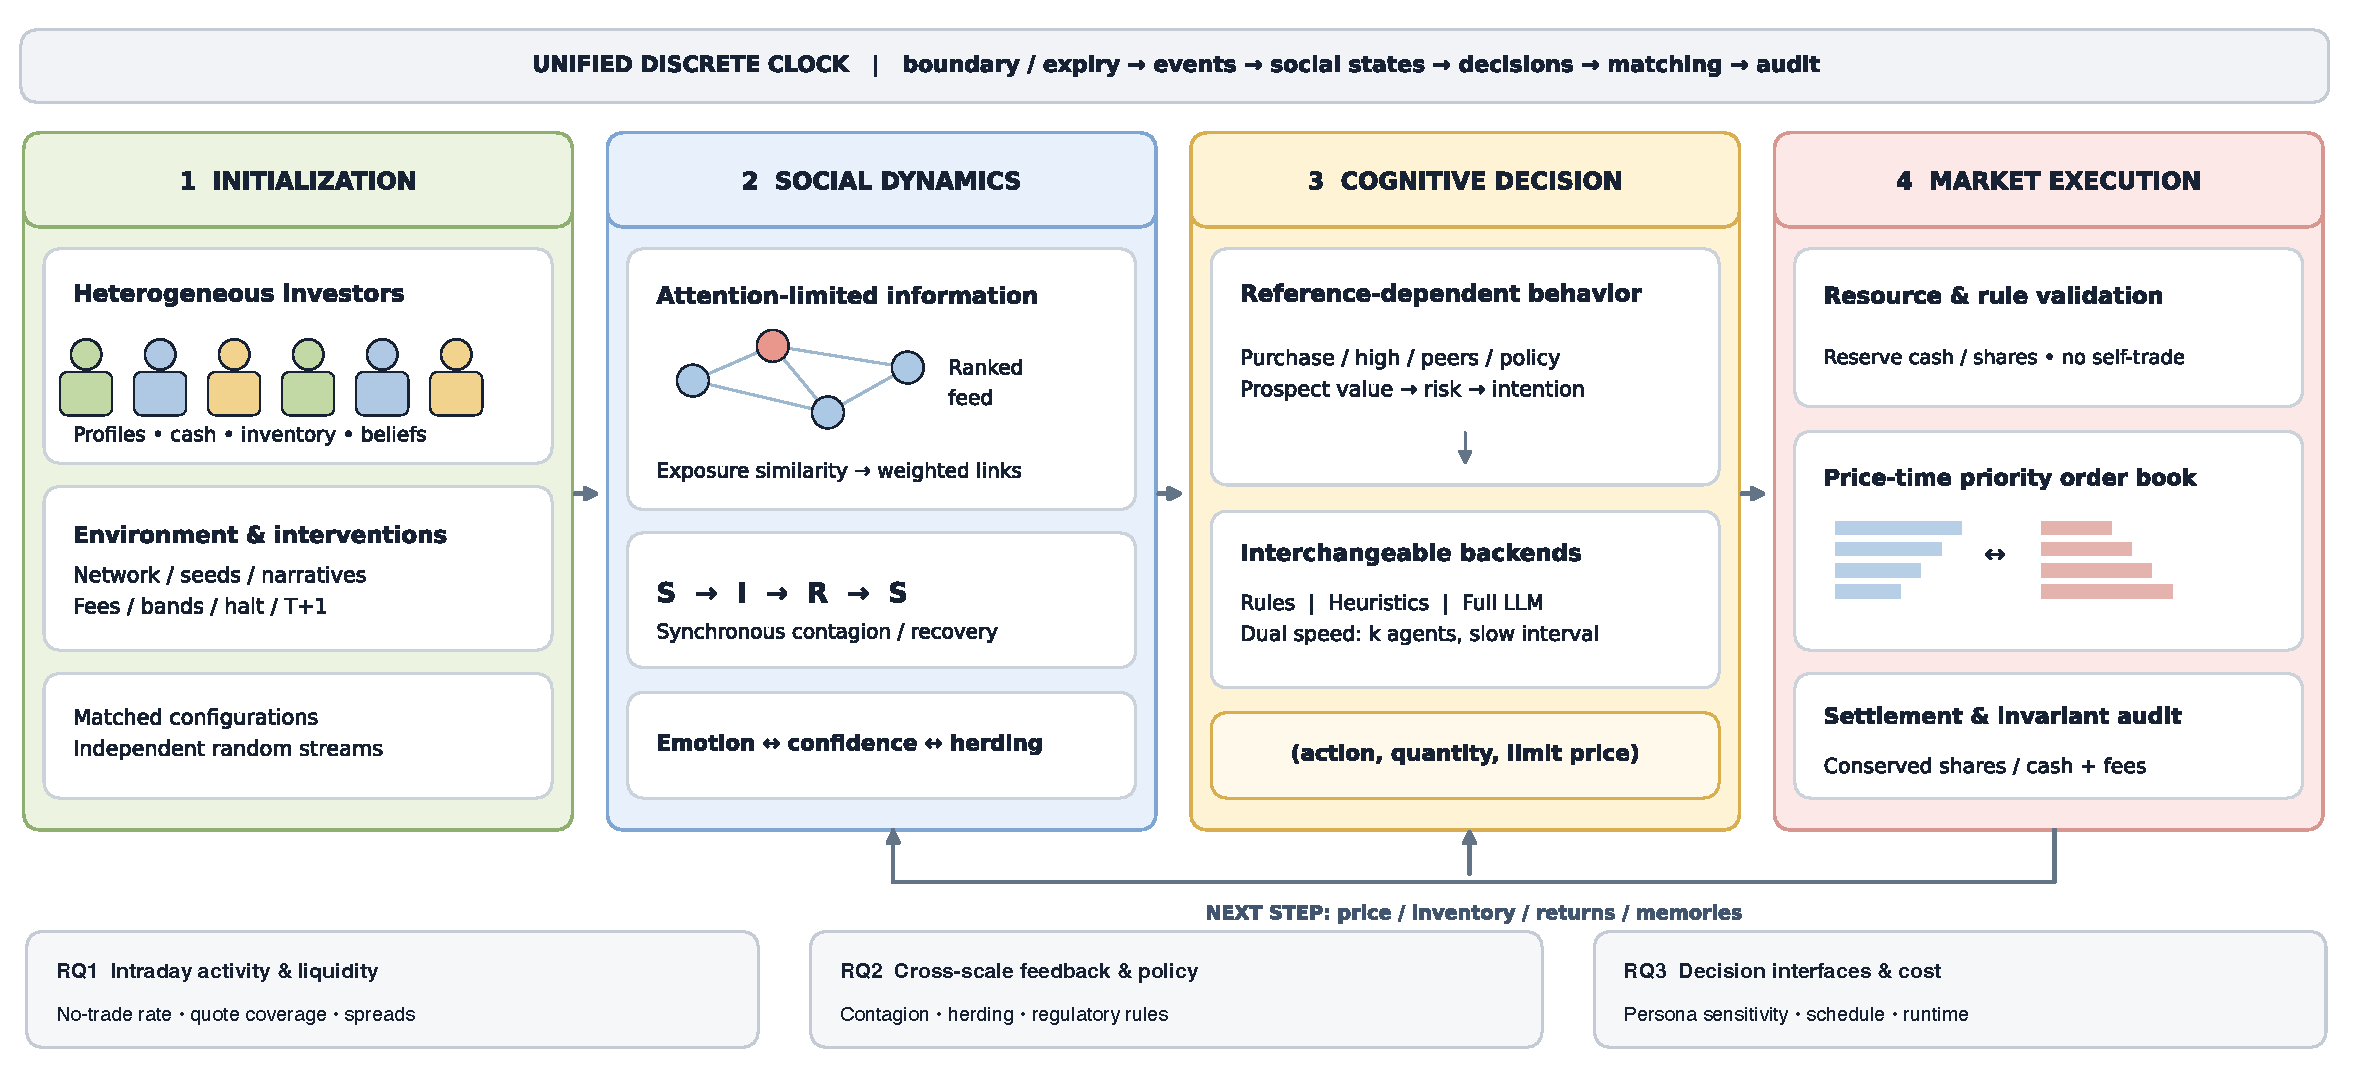
\includegraphics[width=\textwidth]{figures/fig1_methodology_overview.pdf}
  \caption{Civitas Economica 架构。持仓风险暴露调节同伴边权，群体状态参与形成委托，结算产生新的价格和持仓。阶段 \ref{phase:boundary_zh}--\ref{phase:events_zh} 完成市场准备，阶段 \ref{phase:social_zh}--\ref{phase:behavior_zh} 按式~\eqref{eq:exposure_zh}--\eqref{eq:confidence_update_zh} 更新信息与行为状态。阶段 \ref{phase:decision_zh} 通过式~\eqref{eq:aggregate_v_zh}--\eqref{eq:order_quantity_zh} 或认知接口生成委托，接口支持式~\eqref{eq:cache_signature_zh} 的缓存。阶段 \ref{phase:execution_zh}--\ref{phase:commit_zh} 按种子确定的顺序接收委托，并按式~\eqref{eq:settle_b_zh}--\eqref{eq:invariants_zh} 结算与提交。}
  \Description{八阶段时钟连接同伴暴露、群体状态、订单与市场结算，并将结果反馈至下一步，构成三个经济关系尺度。}
  \label{fig:overview}
\end{figure*}

\subsection{统一离散时钟与严格因果调度}
\label{sec:method:clock_zh}

每个仿真步 $t$ 按以下八个阶段推进，以确定各字段何时可见。
\begin{enumerate}[leftmargin=*, label=(\arabic*), ref=\arabic*]
  \item\label{phase:boundary_zh} \textbf{交易日边界与涨跌幅基准重置。} 首日以 $P_0$ 初始化。随后每个交易日首步（$t>1$ 且 $(t-1)\bmod T_{\mathrm{day}}=0$），锚定基准价 $P^{\mathrm{base}}_t = P_{t-1}$，计算日内价格区间 $[P_t^{\mathrm{lower}}, P_t^{\mathrm{upper}}] = [P^{\mathrm{base}}_t(1-L), P^{\mathrm{base}}_t(1+L)]$，并解除到期的持仓锁定。
  \item\label{phase:expiry_zh} \textbf{订单到期与资源释放。} 撤销到期挂单，将剩余预留现金与股份归还可用账本。
  \item\label{phase:events_zh} \textbf{外生事件与公共叙事。} 向公共信息池发布预定的宏观公告、企业财报或监管冲击。
  \item\label{phase:social_zh} \textbf{社会交互与信息筛选。} 按风险暴露相似度更新边权，按注意力容量筛选消息，依据事件处理后的邻居状态同步更新 SIRS 状态。
  \item\label{phase:behavior_zh} \textbf{情绪与信心更新。} 先由上一步信心与悲观邻居占比计算从众权重，再用转移后的感染态、上一步同伴情绪与收益更新 $s_{i,t}$，并按从众触发状态更新信心 $q_{i,t}$。
  \item\label{phase:decision_zh} \textbf{认知决策。} 所有主体均更新参考点。活跃掩码 $A^{\mathrm{act}}_{i,t}\sim\mathrm{Bernoulli}(p_{\mathrm{act}})$ 在主体与步之间抽样，并在匹配比较中共享。活跃主体调用指定后端，输出 \texttt{(action, quantity, price)}，非活跃主体提交 \texttt{HOLD}。
  \item\label{phase:execution_zh} \textbf{订单校验、撮合与结算。} 按共享种子生成的到达顺序处理订单，核验现金或可卖股份。可接受订单在簿内按价格--时间优先撮合，再结算成交和费用。
  \item\label{phase:commit_zh} \textbf{账本审计与状态记录。} 检查现金与股份守恒，记录交易、账本和主体状态。
\end{enumerate}

认知后端接收上一提交步的价格与盘口、当步自身可用资源和心理状态，以及当步已发布事件。自己的执行回执从第 $t+1$ 步可见。单步有效期下，未成交挂单在下一步的阶段（\ref{phase:expiry_zh}）到期，历史盘口作为当步决策的观察值。

\subsection{三层演化尺度与多原型画像}
\label{sec:method:population_zh}

\paragraph{人与人} 点对点联系的权重随风险暴露相似度更新。第 $t-1$ 步结算后，主体 $i$ 的现金与股份分别为 $C_{i,t-1}$ 和 $Q_{i,t-1}$。风险资产暴露定义如下。
\begin{equation}
x^{\mathrm{exp}}_{i,t-1}=\frac{Q_{i,t-1}P_{t-1}}{C_{i,t-1}+Q_{i,t-1}P_{t-1}+\epsilon}.
  \label{eq:exposure_zh}
\end{equation}
主体 $i$ 与邻居 $j$ 的边权向由资产配置相似度决定的目标值平滑更新。
\begin{equation}
\begin{split}w_{ij,t}=\clip\bigl(&(1-\omega)w_{ij,t-1}\\&+\omega(2-|x_i^{\rm exp}-x_j^{\rm exp}|),w_{\min},w_{\max}\bigr).\end{split}
  \label{eq:edge_weight_zh}
\end{equation}
式中 $x_i^{\rm exp}$ 与 $x_j^{\rm exp}$ 均取 $t-1$ 步，$\omega=0.1$，$(w_{\min},w_{\max})=(1,2)$。$\epsilon>0$ 使零财富时的暴露有定义，现金与价格采用同一计价单位。风险敞口越接近，边权的目标值越高。这些边权用于邻域汇总，式~\eqref{eq:message_score_zh} 则在有限注意力下筛选具体消息来源。

\paragraph{人与群体} 筛选后的消息与加权邻域状态经式~\eqref{eq:infection_prob_zh}--\eqref{eq:confidence_update_zh} 更新感染、情绪与信心。九类画像的抽样概率为散户 70\%、公募基金 8\%、养老金 5\%、保险机构 4\%、自营交易台 4\%、做市商 4\%、平准资金 1\%、谣言敏感者 2\% 及套利者 2\%。画像提供角色标签与第~\ref{sec:method:cognition_zh} 节的画像决策参数，并与 Watts--Strogatz 小世界网络独立抽样~\cite{watts1998collective}。这一设置使画像与网络位置可分别调整。各画像的基准损失厌恶系数为 $2.25$。

\paragraph{群体与社会} 这一尺度表示模型市场中的集体结果。各画像的订单在共同交易规则下进入限价订单簿，形成成交价、成交量、报价价差与深度。式~\eqref{eq:settle_b_zh}--\eqref{eq:invariants_zh} 的结算改变持仓，价格与收益进入下一步的暴露、参考点和情绪更新，从而闭合市场结果到个体决策的反馈。

\subsection{社会层：注意力受限传播与信心依赖从众}
\label{sec:method:social_zh}

\paragraph{注意力受限的信息流排名} 设 $\mathcal N_i$ 为主体 $i$ 的邻域。在阶段（\ref{phase:social_zh}），主体对事件处理后处于感染态的邻居消息计算排序分数。
\begin{equation}
\begin{split}h_{ij,t}={}&\theta_1(1-|s_i-s_j|/2)+\theta_2\ind\{u_i=u_j\}\\&+\theta_3(1-|a_i-a_j|)+\theta_4 Inf_j+\theta_5 E_{ij,t-1}.\end{split}
  \label{eq:message_score_zh}
\end{equation}
五项依次为情绪相似度、主题一致性、风险偏好相似度、来源影响力和历史曝光。情绪与风险偏好取上一提交步，非负权重之和为 1。按分数选取至多 $A_i$ 个来源，形成消息集合 $\mathcal F_{i,t}$，同分按固定来源编号排序。

\paragraph{同步 SIRS 恐慌传染动力学} 模型用易感（$S$）、感染（$I$）和恢复（$R$）表示恐慌状态。感染压力由全邻域的加权感染比例与经注意力筛选的消息共同决定。
\begin{equation}
\begin{split}\rho_{i,t}&=\frac{\sum_j w_{ij,t}\ind\{\widetilde X_{j,t}=I\}}{\sum_jw_{ij,t}},\\p^{\rm inf}_{i,t}&=\clip\bigl(\overline{h_{ij,t}\mathrm{sim}_{ij,t}}_{\mathcal F_{i,t}}(\kappa_0+\kappa_1\rho_{i,t})\\&\hspace{5em}+\kappa_2\rho_{i,t},0,1\bigr).\end{split}
  \label{eq:infection_prob_zh}
\end{equation}
其中 $\widetilde X$ 为事件处理后、同步转移前的状态，$\mathrm{sim}_{ij,t}=1-|s_i-s_j|/2$，情绪取上一提交步。$\rho_{i,t}$ 在 $\mathcal N_i$ 内求和，横线表示对 $\mathcal F_{i,t}$ 中各消息的 $h_{ij,t}\mathrm{sim}_{ij,t}$ 取算术平均。空消息集的均值与空邻域的感染比例均置零。易感者以 $\clip(\beta p^{\rm inf}_{i,t}c_i,0,1)$ 的概率感染，$c_i$ 为从众倾向。感染者的恢复概率由当前感染时长和曝光集中度决定。
\begin{equation}
p^{\rm rec}_{i,t}=\clip\bigl(\gamma(1+\eta_d\widetilde D_{i,t})(1-\eta_e e_{i,t}),0,1\bigr).
  \label{eq:recovery_prob_zh}
\end{equation}
曝光记忆按 $E_{ij,t}=(1-\zeta_E)E_{ij,t-1}+\zeta_E\ind\{j\in\mathcal F_{i,t}\}$ 更新，集中度为 $e_{i,t}=\sum_j(E_{ij,t}/\sum_k E_{ik,t})^2$，总曝光为零时取 $e_{i,t}=0$。$\widetilde D$ 为转移前感染时长。恢复者以 $\clip(\delta(1+\eta_\psi p^{\rm inf}_{i,t}),0,1)$ 的概率重返易感态。各主体从转移前状态同步抽样，每步执行至多一次状态转移。

\paragraph{信心依赖的从众反馈} 连续情绪 $s_{i,t}\in[-1,1]$ 由自我惯性、感染状态、同伴情绪和市场收益共同更新。
\begin{equation}
\begin{split}s_{i,t}=\clip\bigl(&(w_i^D-\Delta_{i,t})s_{i,t-1}-w_i^g\ind\{X_{i,t}=I\}\\&+(w_i^N+\Delta_{i,t})\bar s^N_{i,t-1}\\&+w_i^M\clip(r_{t-1}/r_*,-1,1)+\epsilon_s,-1,1\bigr).\end{split}
  \label{eq:sentiment_update_zh}
\end{equation}
同伴情绪为邻居上一步情绪的边权加权均值，孤立主体取自身上一步情绪，$\epsilon_s\sim\mathcal N(0,\sigma_s^2)$。从众反馈在自我惯性和同伴共识之间重新分配权重，保持两者的总权重~\cite{deutsch1955study}。
\begin{equation}
\Delta_{i,t}=H_{i,t}\eta_H(1-q_{i,t-1})w_i^D,\qquad H_{i,t}=\ind\{b^N_{i,t}>0.5\}.
  \label{eq:herding_shift_zh}
\end{equation}
$b^N_{i,t}$ 为情绪低于 $-s_*$ 的邻居所占边权比例。从众触发时信心衰减，其余时间向 $q_0$ 恢复。消融令 $\eta_H=\eta_q=0$，并保留信心恢复项。
\begin{equation}
\begin{split}q_{i,t}=\clip\bigl(&q_{i,t-1}-H_{i,t}\eta_q(1-q_{i,t-1})\\&+(1-H_{i,t})\eta_{\rm rec}(q_0-q_{i,t-1}),0,1\bigr).\end{split}
  \label{eq:confidence_update_zh}
\end{equation}

\subsection{行为核心：多参考点前景理论与订单映射}
\label{sec:method:behavior_zh}

\paragraph{四重自适应参考点} 社会状态更新后，主体在阶段（\ref{phase:decision_zh}）更新持仓成本（$R^p$）、滚动局部高点（$R^h$）、同伴共识（$R^n$）和政策信号（$R^e$）四类心理锚点。
\begin{align}
 R^p_{i,t}&=(1-\kappa_p)R^p_{i,t-1}+\kappa_p T^p_{i,t},\label{eq:ref_p_zh}\\
 R^h_{i,t}&=(1-\kappa_h)R^h_{i,t-1}+\kappa_h \max_{v=\max(0,t-H_h)}^{t-1}P_v,\label{eq:ref_h_zh}\\
 R^n_{i,t}&=(1-\kappa_n)R^n_{i,t-1}+\kappa_nP_{t-1}(1+\xi_n\bar s^N_{i,t-1}),\label{eq:ref_n_zh}\\
 R^e_{i,t}&=(1-\kappa_e)R^e_{i,t-1}+\kappa_eP_{t-1}(1+\xi_e u_t^{\rm policy}).\label{eq:ref_e_zh}
\end{align}
持仓非零时，成本目标为 $T^p=K$，其中 $K$ 为不含费用的持仓成本价。空仓时取 $T^p=P_{t-1}$。政策状态持续至新事件覆盖，事件文本在发布当步可见。

\paragraph{前景价值与动态损失压力} 参考偏差通过非对称幂函数映射为前景价值~\cite{tversky1992advances}。
\begin{equation}
v_i(z)=\begin{cases}z^\alpha&z\ge0,\\-\lambda_i(-z)^\alpha&z<0.\end{cases}
  \label{eq:prospect_v_zh}
\end{equation}
基准设定中 $\lambda_i>1$ 刻画损失厌恶，$\alpha\in(0,1)$ 刻画边际敏感性递减。成本与高点采用回顾性偏差，同伴与政策采用前瞻性偏差。先聚合四类偏差，再计算前景价值与估值方向。
\begin{equation}
\begin{split}x^\bullet_{i,t}&=\begin{cases}(P_{t-1}-R^\bullet_{i,t})/R^\bullet_{i,t}&\bullet=p,h,\\(R^\bullet_{i,t}-P_{t-1})/P_{t-1}&\bullet=n,e,\end{cases}\\z_{i,t}&=\sum_\bullet\omega_\bullet x^\bullet_{i,t},\quad V_{i,t}=v_i(z_{i,t}),\quad d_{i,t}=\tanh(\kappa_vV_{i,t}).\end{split}
  \label{eq:aggregate_v_zh}
\end{equation}
回顾性浮亏比例 $b_{i,t}=(\omega_p\mathbf{1}\{P_{t-1}<R^p_{i,t}\}+\omega_h\mathbf{1}\{P_{t-1}<R^h_{i,t}\})/(\omega_p+\omega_h)$ 衡量价格低于成本或高点的参考权重份额，进入有界的损失压力函数。
\begin{equation}
  \ell_{i,t} = \clip\left( \lambda_i (1 + \chi b_{i,t}), \ell_{\min}, \ell_{\max} \right).
  \label{eq:loss_pressure_zh}
\end{equation}
当前风险偏好 $a_{i,t}\in[0,1]$ 结合信心、上一步风险偏好、情绪、估值方向与损失压力。
\begin{equation}
\begin{split}a_{i,t}=\clip\bigl(&\omega_a^q q_{i,t}+\omega_a^a a_{i,t-1}+\omega_a^s s_{i,t}\\&+\omega_a^d d_{i,t}-\omega_a^\ell\max(0,(\ell_{i,t}-1)/\nu),0,1\bigr).\end{split}
  \label{eq:risk_tolerance_zh}
\end{equation}

\paragraph{交易意图与限价单生成} 估值方向、情绪与风险偏好共同决定交易意图 $\tau_{i,t}\in[-1,1]$。
\begin{equation}
\tau_{i,t}=\clip\bigl(\omega_\tau^d d_{i,t}+\omega_\tau^s s_{i,t}+\omega_\tau^a(a_{i,t}-0.5),-1,1\bigr).
  \label{eq:intent_score_zh}
\end{equation}
在阈值 $\delta_a\ge0$ 下，按以下概率抽样买入、卖出或观望。
\begin{equation}
\begin{split}p_i^b&=\sigma(\kappa_a(\tau_{i,t}-\delta_a)),\\p_i^s&=\sigma(-\kappa_a(\tau_{i,t}+\delta_a)),\qquad p_i^h=1-p_i^b-p_i^s.\end{split}
  \label{eq:action_selection_zh}
\end{equation}
独立随机变量 $U_i\sim U(0,1)$ 决定买入比例 $f_i^b=U_i[f_{\min}+(f_{\max}-f_{\min})a_i]$ 和卖出比例 $f_i^s=U_i[f_{\min}+(f_{\max}-f_{\min})\max(-\tau_i,0)]$。均值校正的对数正态报价扰动独立于动作方向，并在规则基线间共享。
\begin{equation}
\begin{split}\widetilde p_i&=P_{t-1}\exp(\epsilon_p-\sigma_p^2/2),\\p_i^{\rm lim}&=\Delta_p\max\{1,\operatorname{round}_{\rm even}(\widetilde p_i/\Delta_p)\}.\end{split}
  \label{eq:limit_price_zh}
\end{equation}
其中 $\epsilon_p\sim\mathcal N(0,\sigma_p^2)$，刻度取整平局时取偶数，超出当日价带的委托直接拒收。数量按当前可用资源向下取整。
\begin{equation}
  n_i = \begin{cases}
    \bigl\lfloor f^b_{i,t} C_{i,t}^{\mathrm{free}} / \bigl(p_i^{\mathrm{lim}}(1+c)\bigr) \bigr\rfloor & \mathrm{BUY}, \\
    \bigl\lfloor f^s_{i,t} Q_{i,t}^{\mathrm{free}} \bigr\rfloor & \mathrm{SELL}.
  \end{cases}
  \label{eq:order_quantity_zh}
\end{equation}
其中 $c$ 为单侧佣金率，$C^{\rm free}$ 采用与报价一致的元单位。零数量转为 \texttt{HOLD}。

\subsection{市场微观结构与严格守恒审计}
\label{sec:method:microstructure_zh}

\paragraph{资金预留与双向撮合} 买单按限价名义额与买方佣金预留现金，卖单预留可卖股数。账本以每元 $10^6$ 个微元记账，即 $C_{i,t}^{\rm minor}=10^6 C_{i,t}$；成交名义额与费用采用同一微元单位。对整数成交名义额 $V$，每侧佣金为 $f_c=\lfloor cV\rfloor$，卖方印花税为 $f_\tau=\lfloor\tau^{\rm tax}V\rfloor$。

买单按价格降序、卖单按价格升序排列，同价按到达顺序优先，并以已有挂单价格成交。成交 $q^*$ 股时，买方 $b$、卖方 $s$ 与费用账户 $F^{\rm minor}$ 更新为
\begin{align}
  C_b^{\rm minor} &\gets C_b^{\rm minor} - V-f_c, \quad Q_b \gets Q_b + q^*, \label{eq:settle_b_zh} \\
  C_s^{\rm minor} &\gets C_s^{\rm minor} + V-f_c-f_\tau, \quad Q_s \gets Q_s - q^*, \label{eq:settle_s_zh} \\
  F^{\rm minor} &\gets F^{\rm minor} +2f_c+f_\tau. \label{eq:settle_fees_zh}
\end{align}
成交后释放对应成交数量的多余预留，剩余未成交数量的资源继续预留，直至成交、撤销或到期。

\paragraph{账本守恒} 预留资源仍属于账户余额。内核在每个提交步检查主体与费用账户的现金总和，以及主体的股份总量。
\begin{equation}
\begin{aligned}
 \sum_i C_{i,t}^{\rm minor}+F_t^{\rm minor}&=\sum_i C_{i,0}^{\rm minor}+F_0^{\rm minor},\\
 \sum_{i=1}^N Q_{i,t}&=\sum_{i=1}^N Q_{i,0}.
\end{aligned}
  \label{eq:invariants_zh}
\end{equation}
任何非零残差均触发审计错误。

\subsection{认知架构与双速混合调度}
\label{sec:method:cognition_zh}

各后端共享信息字段资格，并输出标准化的 \texttt{(action, quantity, price)}。订单校验和撮合由同一执行内核处理。
\begin{enumerate}[leftmargin=*, label=(\arabic*)]
  \item \textbf{数值规则（System 1）。} 评估公式~(\ref{eq:exposure_zh})--(\ref{eq:order_quantity_zh})，作为规则基线。
  \item \textbf{画像启发式。} 根据估值、趋势与情绪调整各画像的目标持仓比例，并用调整阈值与资源上限决定委托。
  \item \textbf{全量 LLM（System 2）。} 将主体画像、账户状态、市场事实与符合可见条件的记录序列化。接口校验响应身份与动作类型，并检查 \texttt{evidence\_ids} 无重复且属于可见 ID 集合。交易所在执行阶段核验价带与可用资源。
  \item \textbf{双速混合调度。} 全体主体执行轻量的 System 1 状态更新。系统固定选择按画像分层抽样的 $k$ 个主体，在其活跃且 $t\bmod T_{\mathrm{slow}}=0$ 时请求 System 2 响应。
\end{enumerate}

市场运行器执行规则决策、受控合成响应和归档响应。真实模型请求通过独立的固定观察工具测试同一决策契约。

\paragraph{资源自适应策略缓存} System 2 请求步缓存标准化方向与资源承诺比例，使后续订单适应当步价格和余额。
\begin{equation}
\begin{aligned}
 \widehat d_i &=
 \begin{cases}
   +1 & \mathrm{BUY}, \\
   -1 & \mathrm{SELL}, \\
   0 & \mathrm{HOLD},
 \end{cases} \\
 \widehat f_i &=
 \begin{cases}
   \min\!\bigl(1,n_i/M_i^{\mathrm{action}}\bigr) & M_i^{\mathrm{action}}>0, \\
   0 & \mbox{其他情况。}
 \end{cases}
\end{aligned}
  \label{eq:cache_signature_zh}
\end{equation}
其中 $M_i^{\mathrm{action}}$ 为按请求限价和连续佣金预算界计算的保守容量，\texttt{HOLD} 的资源承诺为零。复用时，活跃主体保持 $\widehat d_i$ 与 $\widehat f_i$，以共同报价扰动围绕 $P_{t'-1}$ 生成新限价，再将承诺比例乘以当前容量并向下取整。缓存可在年龄 $1$ 至 $A_{\max}$ 步间复用，含两端。缺失或过期时使用规则后端。已知响应异常清除缓存并提交 \texttt{HOLD}；复用后的最终数量为零时也提交 \texttt{HOLD}。

\paragraph{模型请求的调度预算} 全量 LLM 调度在 $T$ 步内提供的期望请求机会为 $p_{\mathrm{act}}NT$，双速调度为 $p_{\mathrm{act}}k\lfloor T/T_{\mathrm{slow}}\rfloor$。两者之比近似为
\begin{equation}
  \text{请求机会比} \approx \frac{k}{N \cdot T_{\mathrm{slow}}}.
  \label{eq:cost_ratio_zh}
\end{equation}
当 $N=100$、$k=10$、$T_{\rm slow}=10$ 且期限为周期整数倍时，期望请求机会减少 99\%。首个请求窗口在 $T_{\rm slow}$，固定周期调度只在预定窗口请求。实测成本按实际用量和耗时统计。
\paragraph{分析工具} OpenAI Codex 辅助实现与公式比对、归档核对和稿件整理。论文的实测分析与图表依据可追溯的归档记录。
